\section{Work plan — Work packages, deliverables}

The present section accounts for an accurate description of the different steps and milestones that need to be accomplished by DEOS-UD in order to succeed in the development of the project. The reader will find here information related with the overall structure of the project, the different Work Packages and their timings along with the list of deliverables and milestones expected for the project. In addition to the information described, an approach to the interrelation between components will be displayed in order for the reader to better understand the complexity of the project.  

\subsection{Overall Structure}
%Brief presentation of the overall structure of the work plan. \textbf{Network diagram SOLO de los WP o diagrama explicativo del proyecto. El network diagram que tenemos ahora está en D2 Apartado 3.2.}

The DEOS-UD project is composed by 7 different work packages which are interrelated as shown in Figure \ref{overallstructure}. WP1 deals with project management and will ensure the proper coordination of project activities and the achievement of project objectives. WP2 is related to the quality and the administration of the project in terms of human resources, documentation management and quality, periodic monitoring and will also establish the financial plan of the project. WP3 will study the current baseline designs for the studied technologies (payload, modular system and urban development application) in the sector and will establish the potential areas of improvement and the requirements that need to be achieved by the new technologies proposed. WP4 is in charge of designing the output products of the project. This WP is strongly related to WP5, which is in charge of manufacturing and validating the prototype. Good intercommunication between these WPs is needed in order to obtain a final product that meets the requirements imposed by WP3. WP6 aims to create a methodology to enable the future use of the new technologies developed during the project, assuring their continuity. Finally, WP7 will ensure the project results are communicated and disseminated to the appropriate audiences, establishing this new knowledge into the society. 

\begin{figure}[H]
\centering
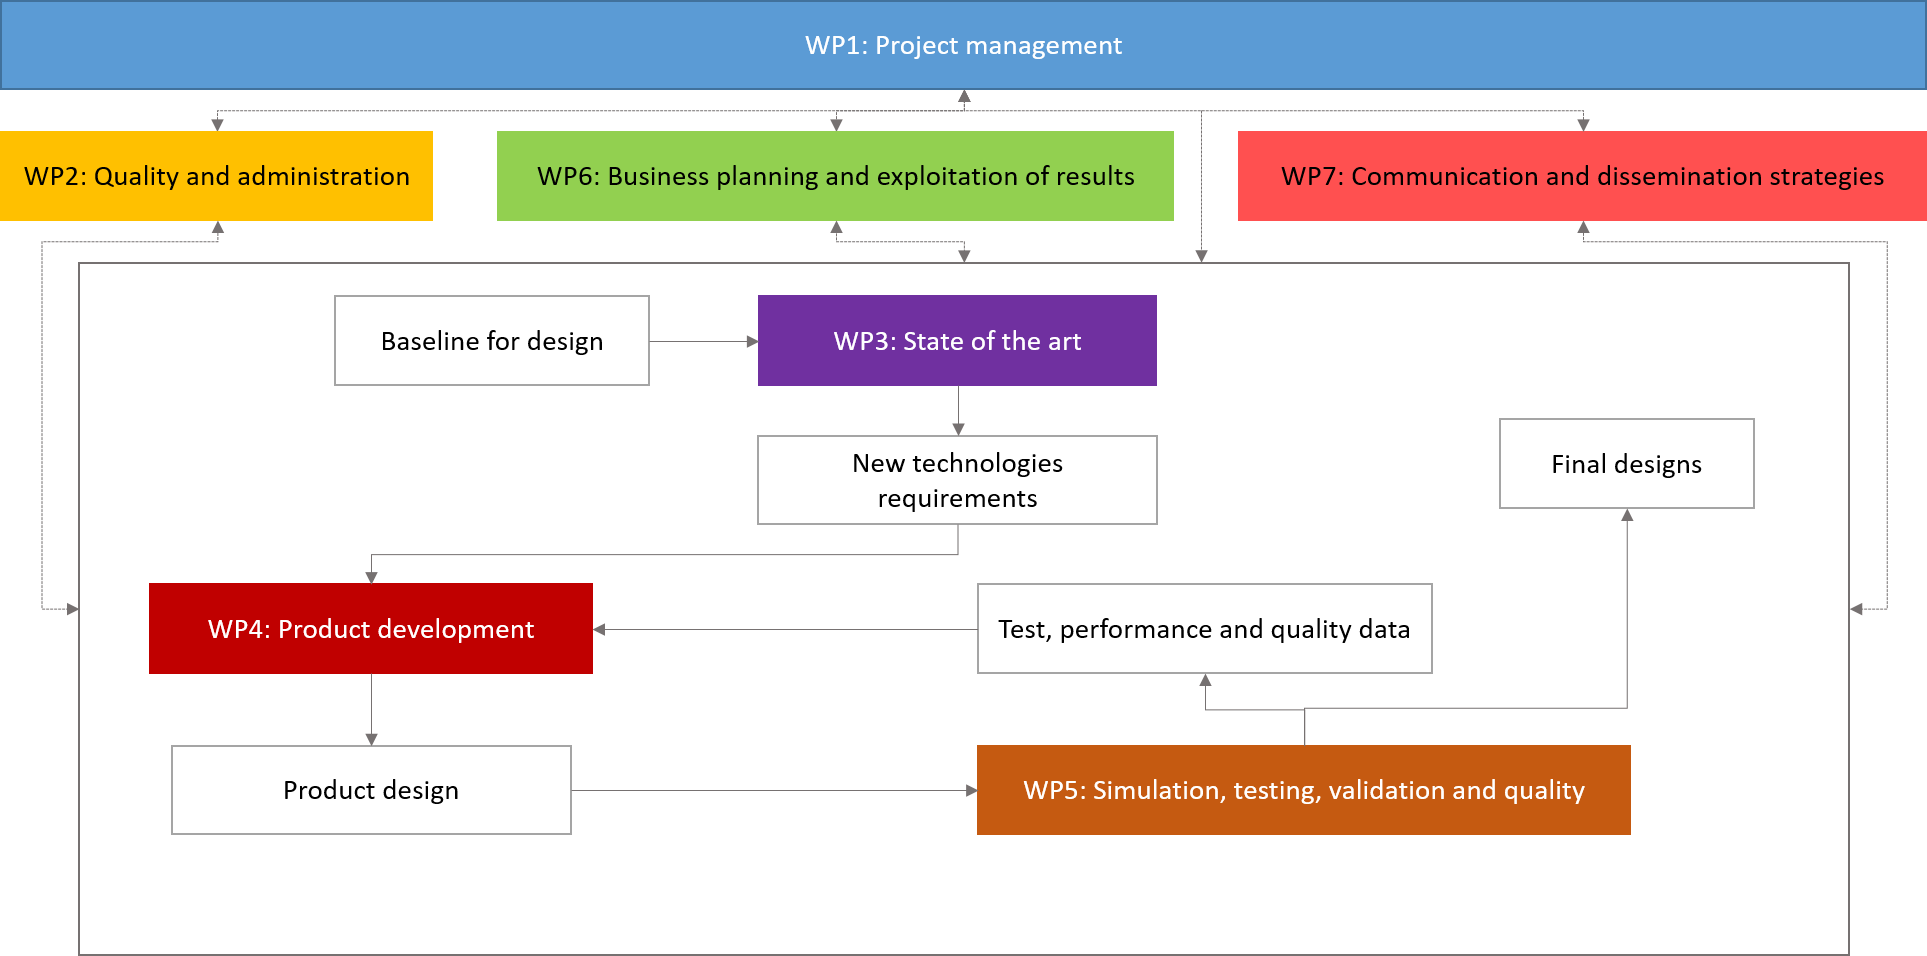
\includegraphics[width=\textwidth]{images/overallstructure.png}
\caption{DEOS-UD overall structure diagram.} 
\label{overallstructure}
\end{figure}

\subsection{Timing of the Work Plan}

The following Gantt diagram contains all the tasks planned for the project, with their chronological order and duration. The Gantt diagram serves as a base for the project resource planning and time management.

\begin{landscape}
	\begin{figure}[H]
	\centering
	\begin{tabular}{@{}c@{\hspace{.5cm}}c@{}}
		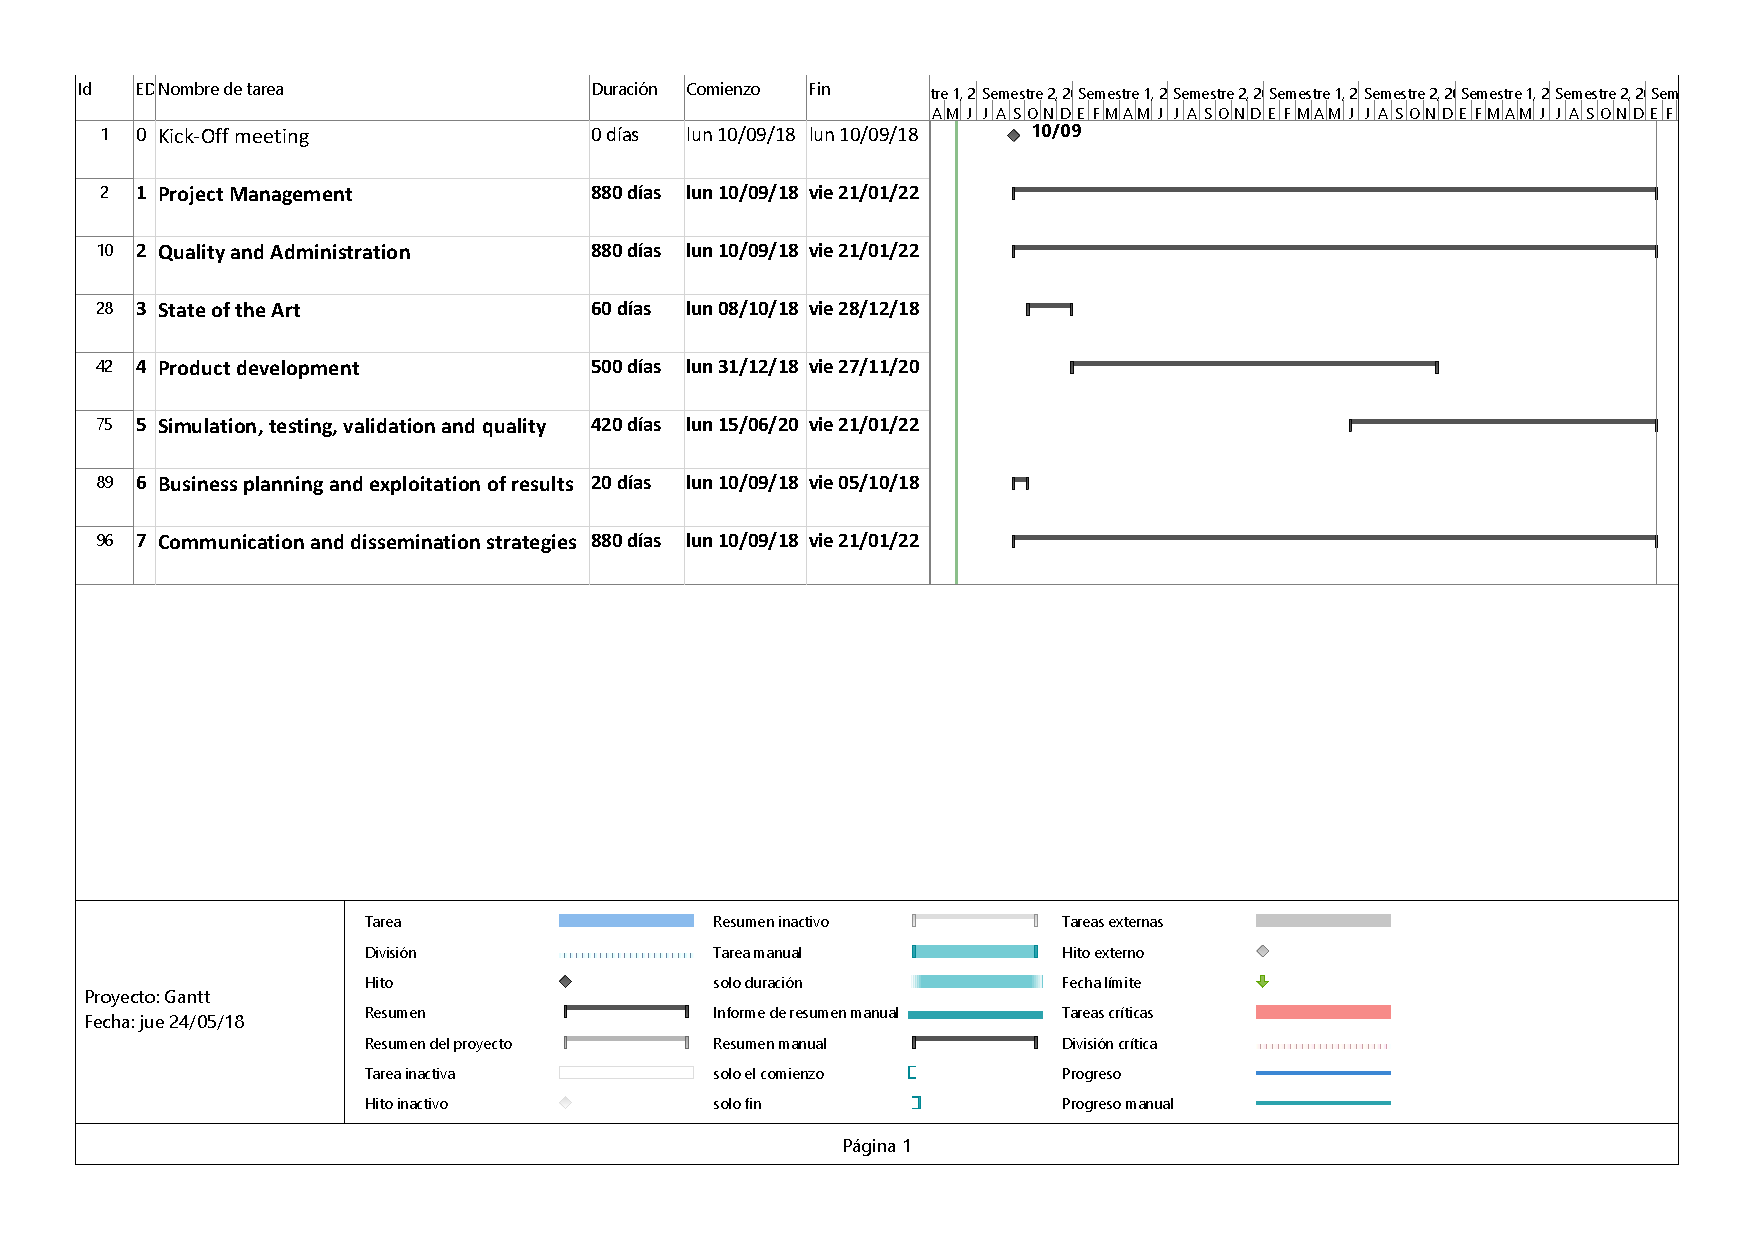
\includegraphics[page=1,width=1.2\textwidth]{./pdf/GANTT.pdf}
	\end{tabular}
	\caption{Gantt chart}
	\label{Gantt}
	\end{figure}
\end{landscape}

\subsection{Description of Work Packages}

%\begin{itemize}

%\item List of WP. \textbf{D2 Apartado 2.1 Poner solo WP, no todas las activities. Extraer del D2 también Start Month i End Month}

%\item Description of each WP. \textbf{Extraer información de D2 sección 2 (Número de participantes, líder, objetivos, etc.) Hay que poner las diferentes tareas dentro de cada WP y quienes participan en cada tarea. Importante: Falta calcular PM por participante. Deliverables asociados a cada WP ( también a extraer del D2).}

%\end{itemize}

% \usepackage{array} is required

\begin{table}[H]
	\centering
	\begin{tabular}{p{1.4cm} >{\raggedright\arraybackslash}p{2.7cm} p{1.8cm} p{2.2cm} p{1.3cm} p{1.2cm} p{1.3cm}}
	
		\toprule[2pt]
		
		\textbf{Work Package No.} & \textbf{Work Package Title} & \textbf{Lead Participant No.} & \textbf{Lead Participant Short Name} & \textbf{Person Months} & \textbf{Start Month} & \textbf{End Month} \\
		
		\midrule[1.5pt] 
		
		 1& Project management & 4 & HR & 16 & M1 & M44 \vspace{0.2cm} \\
		
		\midrule
	
		 2& Quality and administration & 4 & HR &  26 & M1 & M44 \vspace{0.2cm} \\
		
		\midrule
		
		 3& State of the art & 1 & ADS & 34 & M1 & M3 \vspace{0.2cm} \\
	
		\midrule
	
	 	 4& Product development & 1 & ADS & 119 & M4 & M29 \vspace{0.2cm} \\
	 	 
	 	 \midrule
	 	 
	 	 5& Simulation, testing, validation and quality & 7 & TAS & 27 & M22  & M43 \vspace{0.2cm} \\
	 	 
	 	 \midrule
	 	 
	 	 6& Business planning and exploitation of results & 2 & BHO & 16 & M1 & M2 \vspace{0.2cm} \\
	 	 
	 	 \midrule
	 	 
	 	 7& Communication and dissemination strategies & 4 & HR & 21 & M1 & M44 \vspace{0.2cm} \\
		
		\bottomrule[2pt]
	
	\end{tabular}
	\caption{List of work packages}
	\label{workpackages}
\end{table}

\pagebreak

\begin{center}
	
\begin{longtable}{| >{\raggedright\arraybackslash}p{3cm} | >{\raggedright\arraybackslash}m{1cm} | >{\raggedright\arraybackslash}m{1cm} | >{\raggedright\arraybackslash}m{1cm}| >{\raggedright\arraybackslash}m{1cm}| >{\raggedright\arraybackslash}m{1cm} | >{\raggedright\arraybackslash}m{1cm} |>{\raggedright\arraybackslash}m{1cm}|>{\raggedright\arraybackslash}m{1cm}| }
		
		\hline
		\multicolumn{4}{|>{\raggedright\arraybackslash}l|}{\textbf{Work Package Number:}  1}&\multicolumn{5}{|>{\raggedright\arraybackslash}l|}{\textbf{Lead beneficiary:}  HIRO}\\
		
		\hline
		
		\multicolumn{9}{|>{\raggedright\arraybackslash}l|}{\textbf{Work Package Title:} Project management }\\
		
		\hline 
		
		\textbf{Participant number}&1&2&3&4&5&6&7&8\\
		
		\hline
		
		\textbf{Short name of participant}& ADS & BHO & DS & HR& IS & RSAC & TAS & VT\\
		 
		 \hline 
		 
		 \textbf{Person Month per Participant}&0&0&0&16&0&0&0&0\\
		 
		 \hline
		 
		 \multicolumn{4}{|>{\raggedright\arraybackslash}l|}{\textbf{Start Month}  M1}&\multicolumn{5}{|>{\raggedright\arraybackslash}l|}{\textbf{End month:}  M44}\\
		 
		 \hline
		
		\multicolumn{9}{|>{\raggedright\arraybackslash}l|}{\parbox[t]{14cm}{\textbf{Objectives:} \newline
		 The aim of WP1 is to ensure a good coordination and management of the project covering technical, administrative, ethical and financial issues. The specific aims are:
\begin{itemize}
\item Coordinate DEOS-UD project providing the partners with the needed organization, supervision and leadership.
\item Manage and monitor the project progress.
\item Understand the overall project together with its risk and determination of mitigation and contingency plans for the proper development of the project.
\end{itemize}
		
		}}\\
		
		\hline 
		 
		 \multicolumn{9}{|>{\raggedright\arraybackslash}l|}{\parbox[t]{14cm}{\textbf{Description of work:} \newline 
		 
\underline{Task 1.1: Development of project management plan.} \textit{Leadership: HR}. Elaboration of all the documentation that states the strategy of the management and organization of the project through its duration.\\

\underline{Task 1.2: Monitoring of the project.} \textit{Leadership: HR}. Gathering of the members of the project to inform
each other of the progress. Tracking of the active tasks and scheduling.\\

\underline{Task 1.3: Annual reporting.} \textit{Leadership: HR}. Every year that the project lasts will call for the
elaboration of an internal report with the aim of
keeping up to date with the progress done.\\

\underline{Task 1.4: Project implementation of risk management.} \textit{Leadership: HR}. Study of all the potential risks and how will they
be managed so that their affectation to the project
stays to a minimum.\\

		 
		 }}\\
		 \hline 
		 
		 \multicolumn{9}{|>{\raggedright\arraybackslash}l|}{\parbox[t]{14cm}{\textbf{Deliverables:} \newline \underline{D1.1: Project management plan:} Document with detailed explanation
of the project management strategies,
including the Project Charter,
stakeholder register, risk, quality and
financial plans. Due date: M1\\

\underline{D1.2: Final Report:} Final document delivered, that includes all the development done through the execution of the project.\\

}}\\
		 
		 \hline 
		 
		%\end{tabular}
		
		\caption{WP1 description}
		
\end{longtable}


\begin{table}[H]
\begin{tabular}{| >{\raggedright\arraybackslash}p{3cm} | >{\raggedright\arraybackslash}m{1cm} | >{\raggedright\arraybackslash}m{1cm} | >{\raggedright\arraybackslash}m{1cm}| >{\raggedright\arraybackslash}m{1cm}| >{\raggedright\arraybackslash}m{1cm} | >{\raggedright\arraybackslash}m{1cm} |>{\raggedright\arraybackslash}m{1cm}|>{\raggedright\arraybackslash}m{1cm}| }
		
		\hline
		\multicolumn{4}{|>{\raggedright\arraybackslash}l|}{\textbf{Work Package Number:}  2}&\multicolumn{5}{|>{\raggedright\arraybackslash}l|}{\textbf{Lead beneficiary:}  HIRO}\\
		
		\hline
		
		\multicolumn{9}{|>{\raggedright\arraybackslash}l|}{\textbf{Work Package Title:} Quality and administration }\\
		
		\hline 
		
		\textbf{Participant number}&1&2&3&4&5&6&7&8\\
		
		\hline
		
		\textbf{Short name of participant}&ADS&BHO&DS&HR&IS&RSAC&TAS&VT\\
		 
		 \hline 
		 
		 \textbf{Person Month per Participant}&0&11&15&0&0&0&0&0\\
		 
		 \hline
		 
		 \multicolumn{4}{|>{\raggedright\arraybackslash}l|}{\textbf{Start Month}  M0}&\multicolumn{5}{|>{\raggedright\arraybackslash}l|}{\textbf{End month:}  M44}\\
		 
		 \hline
		
		\multicolumn{9}{|>{\raggedright\arraybackslash}l|}{\parbox[t]{14cm}{\textbf{Objectives:} \newline The aim of WP2 is to manage the human resources of the project in order to supply the amount of them needed to perform the project. It is also in charge of developing and controlling the financial feasibility study and seek funding to achieve the project objectives. Documentation management and periodic monitoring will also be done in this WP, assuring the quality of the deliverables and other documentation.\\
		 
		}}\\
		
		\hline 
		 
		 \multicolumn{9}{|>{\raggedright\arraybackslash}l|}{\parbox[t]{14cm}{\textbf{Description of work:} \newline 
\underline{Task 2.1: Human resources.} \textit{Leadership: HR}. Definition of the number of employees necessary and employment of them. Administration of all the employees needed to fulfill the different tasks of the project.\\

\underline{Task 2.2: Financial plan.} \textit{Leadership: HR}. Lay down of all the fix and variable costs of the project and the expected funding. Study on the economic feasibility of the project, monitoring of the evolution of the project finances and search for the additional funding for the project. \\

\underline{Task 2.3: Documentation management.} \textit{Leadership: HR}. Establishment of the guidelines for the redaction of all documents, revision of all the documents of the project and rectification of the documents that do not meet the project requirements. Approval of the reviewed and rectified documents. \\

\underline{Task 2.4: Periodic monitoring.} \textit{Leadership: HR}. To ensure the quality of the project, a periodic monitoring of all the activities will be carried out.\\
	 
		 }}\\
		 \hline 
		 
		 \multicolumn{9}{|>{\raggedright\arraybackslash}l|}{\parbox[t]{14cm}{\textbf{Deliverables:} \newline 
\underline{D2: Quality and Administration plan:} Document with detailed explanation of the project quality and administration plan that will be elaborated before the design and manufacturing stages start in order to assure the quality of the processes. Due date: M1.\\

}}\\
		 
		 \hline 
		 
		\end{tabular}
		
		\caption{WP2 description}
		
\end{table}


\begin{table}[H]
\begin{tabular}{| >{\raggedright\arraybackslash}p{3cm} | >{\raggedright\arraybackslash}m{1cm} | >{\raggedright\arraybackslash}m{1cm} | >{\raggedright\arraybackslash}m{1cm}| >{\raggedright\arraybackslash}m{1cm}| >{\raggedright\arraybackslash}m{1cm} | >{\raggedright\arraybackslash}m{1cm} |>{\raggedright\arraybackslash}m{1cm}|>{\raggedright\arraybackslash}m{1cm}| }
		
		\hline
		\multicolumn{4}{|>{\raggedright\arraybackslash}l|}{\textbf{Work Package Number:}  3}&\multicolumn{5}{|>{\raggedright\arraybackslash}l|}{\textbf{Lead beneficiary:} \newline
		 \begin{tabular}[c]{@{}l@{}}Airbus Defence and \\  Space \end{tabular}}\\
		
		\hline
		
		\multicolumn{9}{|>{\raggedright\arraybackslash}l|}{\textbf{Work Package Title:} State of the art }\\
		
		\hline 
		
		\textbf{Participant number}&1&2&3&4&5&6&7&8\\
		
		\hline
		
		\textbf{Short name of participant}&ADS&BHO&DS&HR&IS&RSAC&TAS&VT\\
		 
		 \hline 
		 
		 \textbf{Person Month per Participant}&8&0&3&3&6&4&6&4\\
		 
		 \hline
		 
		 \multicolumn{4}{|>{\raggedright\arraybackslash}l|}{\textbf{Start Month}  M1}&\multicolumn{5}{|>{\raggedright\arraybackslash}l|}{\textbf{End month:}  M3}\\
		 
		 \hline
		
		\multicolumn{9}{|>{\raggedright\arraybackslash}l|}{\parbox[t]{14cm}{\textbf{Objectives:} \newline The aim of WP3 is to do a state of the art for the technologies that want to be studied and improved during the project. The final objective is being capable of seeing the possibilities of these technologies and the potential areas of improvement to specify the requirements needed to achieve by the next-generation sensors, systems and applications.\\
		 
		}}\\
		
		\hline 
		 
		 \multicolumn{9}{|>{\raggedright\arraybackslash}l|}{\parbox[t]{14cm}{\textbf{Description of work:} \newline 
		\underline{Task 3.1: Payloads.} \textit{Leadership: ADS. Participants: DS, TAS and HR.} Search for the current space applications and definition of the requirements for the sensors.\\
		
		\underline{Task 3.2: Modular system.} \textit{Leadership: TAS. Participants: DS, ADS and HR.} Search for the current modular systems with space applications and definition of the requirements for the modular system developed in the project.\\
		
		\underline{Task 3.3: Urban development applications with space technologies.} \textit{Leadership: IS. Participands: VT, RSAC and HR.} Search for current applications similar to those that want to be implemented in this project in the areas of weather forecast, urban planning and greenhouse emissions reduction. Definition of the requirements of the applications.\\
		 }}\\
		 \hline 
		 
		 \multicolumn{9}{|>{\raggedright\arraybackslash}l|}{\parbox[t]{14cm}{\textbf{Deliverables:} \newline 
		 \underline{D3.1: Payload state of the art:} Report containing the state of the art of current EO remote
sensors as well as the sensors to improve selection and the first
requirements definition. Due date: M4\\

\underline{D3.2: Modular system state of the art: }Report containing the state of the art of current modular
systems with space applications and its first requirements
definition. Due date: M4\\

\underline{D3.3: Space applications state of the art:} Report containing the state of the art of current urban
development space applications and first interaction platforms
requirements definition. Due date: M4\\
}
              }\\
		 
		 \hline 
		 
		\end{tabular}
		
		\caption{WP3 description}
		
\end{table}



%\begin{table}[H]
\begin{longtable}{| >{\raggedright\arraybackslash}p{3cm} | >{\raggedright\arraybackslash}m{1cm} | >{\raggedright\arraybackslash}m{1cm} | >{\raggedright\arraybackslash}m{1cm}| >{\raggedright\arraybackslash}m{1cm}| >{\raggedright\arraybackslash}m{1cm} | >{\raggedright\arraybackslash}m{1cm} |>{\raggedright\arraybackslash}m{1cm}|>{\raggedright\arraybackslash}m{1cm}| }
		
		\hline
		\multicolumn{4}{|>{\raggedright\arraybackslash}l|}{\textbf{Work Package Number:}  4}&\multicolumn{5}{|>{\raggedright\arraybackslash}l|}{\textbf{Lead beneficiary:} \newline
		 \begin{tabular}[c]{@{}l@{}}Airbus Defence and \\  Space \end{tabular}}\\
		
		
		\hline
		
		\multicolumn{9}{|>{\raggedright\arraybackslash}l|}{\textbf{Work Package Title:} Product development }\\
		
		\hline 
		
		\textbf{Participant number}&1&2&3&4&5&6&7&8\\
		
		\hline
		
		\textbf{Short name of participant}&ADS&BHO&DS&HR&IS&RSAC&TAS&VT\\
		 
		 \hline 
		 
		 \textbf{Person Month per Participant}&40&0&10&6&25&5&25&8\\
		 
		 \hline
		 
		 \multicolumn{4}{|>{\raggedright\arraybackslash}l|}{\textbf{Start Month}  M4}&\multicolumn{5}{|>{\raggedright\arraybackslash}l|}{\textbf{End month:}  M29}\\
		 
		 \hline
		
		\multicolumn{9}{|>{\raggedright\arraybackslash}l|}{\parbox[t]{14cm}{\textbf{Objectives:} \newline The aim of WP4 is to do the design of the sensors and systems that will be created by the project. This include the three main branches of the project: sensor, modular system and data application for urban development. A preliminary design according to the specified requirements will be done and then, based on simulations and testing, the final design will be created. \\
		
		}}\\
		
		\hline 
		 
		 \multicolumn{9}{|>{\raggedright\arraybackslash}l|}{\parbox[t]{14cm}{\textbf{Description of work:} \newline 
		\underline{Task 4.1: Preliminary design.} \textit{Leadership: ADS. Participants: DS, TAS, HR, VT, RSAC, IS}. Research for the payload preliminary design and development of it. Modular system preliminary design, definition of SATCOM application domains and development of: physical framework for sensor block, systems interactions and applications, sensor data fusion software. Preliminary design of the interaction platform and implementation of web-based servers for sharing sensors data and processing algorithms based on applications.\\
		 
		\underline{Task 4.2: Final design:} \textit{Leadership: ADS. Participants: DS, TAS, HR, VT, RSAC, IS}. Final design and technical specifications of the payload sensors. Final design of the modular system, specifically the sensors data fusion software. Final design and implementation of the interaction platform, including the web servers for data sharing and the processing algorithms. \\
		
		
		 }}\\
		 \hline 
		 
		 \multicolumn{9}{|>{\raggedright\arraybackslash}l|}{\parbox[t]{14cm}{\textbf{Deliverables:} \newline 
		 \underline{D4.1 Payload preliminary design:} Report determining the payload preliminary design. It contains
the research, requirements and preliminary performances
parameters of each sensor.\\

		 \underline{D4.2 Modular system preliminary design:} Report detailing the modular system preliminary design. It
includes a first review of the sensors blocks physical framework
and sensors data fusion software requirements as well as the
initial definition of the SATCOM application domains.\\

		 \underline{D4.3 Interaction platform preliminary design:} Report detailing the interaction platform preliminary design. It
includes the predesign of data sharing servers and platforms
as well as the definition of the initial implementation of data
processing algorithms.\\

		 \underline{D4.4 Payload final design:} Report detailing the final design and technical specifications of
each developed sensor.\\

		 \underline{D4.5 Modular system final design:} Report detailing the final design and technical specifications of
the modular system.\\

		 \underline{D4.6 Sensor data fusion software report:} Report containing the final sensors data fusion software
specifications.\\

		 \underline{D4.7 Interaction platform final design:} Report containing the final design and technical specifications
of the interaction platforms.\\

		 \underline{D4.8 Data processing software report:} Report containing the final data processing algorithms
specifications which will allow processing the acquired satellite
data.\\

		 
		 
		 }}\\
		 
		 \hline 
		 
		%\end{tabular}
		
		\caption{WP4 description}
		
\end{longtable}

%%%%%%%%%%%%%%%%%%%%%%%%%%%%%%%%%%%%%%%%%%%%%%%%%%%%%%% WP5

\begin{longtable}[H]{| >{\raggedright\arraybackslash}p{3cm} | >{\raggedright\arraybackslash}m{1cm} | >{\raggedright\arraybackslash}m{1cm} | >{\raggedright\arraybackslash}m{1cm}| >{\raggedright\arraybackslash}m{1cm}| >{\raggedright\arraybackslash}m{1cm} | >{\raggedright\arraybackslash}m{1cm} |>{\raggedright\arraybackslash}m{1cm}|>{\raggedright\arraybackslash}m{1cm}| }
		
		\hline
		\multicolumn{4}{|>{\raggedright\arraybackslash}l|}{\textbf{Work Package Number:}  5}&\multicolumn{5}{|>{\raggedright\arraybackslash}l|}{\textbf{Lead beneficiary:} \newline
		 \begin{tabular}[c]{@{}l@{}}Thales Alenia Space \\  S.A.S \end{tabular}}\\
		
		\hline
		
		\multicolumn{9}{|>{\raggedright\arraybackslash}l|}{\textbf{Work Package Title:} Simulation, testing, validation and quality }\\
		
		\hline 
		
		\textbf{Participant number}&1&2&3&4&5&6&7&8\\
		
		\hline
		
		\textbf{Short name of participant}&ADS&BHO&DS&HR&IS&RSAC&TAS&VT\\
		 
		 \hline 
		 
		 \textbf{Person Month per Participant}&5&0&3&4&1&4&8&2\\
		 
		 \hline
		 
		 \multicolumn{4}{|>{\raggedright\arraybackslash}l|}{\textbf{Start Month}  MX}&\multicolumn{5}{|>{\raggedright\arraybackslash}l|}{\textbf{End month:}  MX}\\
		 
		 \hline
		
		\multicolumn{9}{|>{\raggedright\arraybackslash}l|}{\parbox[t]{14cm}{\textbf{Objectives:} \newline The aim of WP5 is to manufacture and validate the sensors designed. This includes the manufacture, simulation, testing and validation of all the products developed in the three main branches of the project ensuring the quality of the product. \\
		}}\\
		
		\hline 
		 
		 \multicolumn{9}{|>{\raggedright\arraybackslash}l|}{\parbox[t]{14cm}{\textbf{Description of work:} \newline 
		\underline{Task 5.1: Technology Demonstrator Prototype Manufacturing.} \textit{Leadership: TAS. Participants: ADS, DS, HR}. Manufacturing of the sensors, the module and the interaction platform of the prototype in order to be tested in the following activities.\\
		 
		\underline{Task 5.2: Payload Validation.} \textit{Leadership: TAS. Participants: ADS, DS, HR}. Validation of the performance of the sensors mounted on the system. \\

		\underline{Task 5.3: Modular System Validation.} \textit{Leadership: TAS. Participants: ADS, DS, HR}. Validation of the modular system performance, of the systems interaction, of the sensors data fusion software, of the satellite communications applications domains and also of the physical framework for sensor blocks.\\

		\underline{Task 5.4: Interaction Platform Validation.} \textit{Leadership: RSAC. Participants: HR, VT, IS}. Validation of the interaction platform to check if it develops all its functions properly.\\

		\underline{Task 5.5: Full System Prototype Validation.} \textit{Leadership: HR. Participants: ADS, TAS, RSAC}. Validation of the whole system using the prototype in order to test its performance.\\

		\underline{Task 5.6: Quality of the Product.} \textit{Leadership: HR. Participants: DADS, TAS, RSAC}. Quality control of all the subsystems of the product and all the methodologies applied on its manufacturing and validation.\\
		
		 }} \\
		 \hline 
		 
		 \multicolumn{9}{|>{\raggedright\arraybackslash}l|}{\parbox[t]{14cm}{\textbf{Deliverables:} \newline 
		 \underline{D5 Validation Report:} Report that gathers the tests and validations with the obtained results of all the payload sensors, the modular system and the interaction platform, as well as the full system performing. \\
		 }}\\
		 
		 \hline 
		 
		%\end{tabular}
		
		\caption{WP5 description}
		
\end{longtable} 

%%%%%%%%%%%%%%%%%%%%%%%%%%%%%%%%%%%%%%%%%%%%%%%%%%%%%%% WP6

\begin{table}[H]
\begin{tabular}{| >{\raggedright\arraybackslash}p{3cm} | >{\raggedright\arraybackslash}m{1cm} | >{\raggedright\arraybackslash}m{1cm} | >{\raggedright\arraybackslash}m{1cm}| >{\raggedright\arraybackslash}m{1cm}| >{\raggedright\arraybackslash}m{1cm} | >{\raggedright\arraybackslash}m{1cm} |>{\raggedright\arraybackslash}m{1cm}|>{\raggedright\arraybackslash}m{1cm}| }
		
		\hline
		\multicolumn{4}{|>{\raggedright\arraybackslash}l|}{\textbf{Work Package Number:}  6}&\multicolumn{5}{|>{\raggedright\arraybackslash}l|}{\textbf{Lead beneficiary:} \newline
		 \begin{tabular}[c]{@{}l@{}}BHO Legal \\ PRechtsanwalte \\ Partnership\end{tabular}}\\
		
		\hline
		
		\multicolumn{9}{|>{\raggedright\arraybackslash}l|}{\textbf{Work Package Title:} Business planning and exploitation of results} \\
		
		\hline 
		
		\textbf{Participant number}&1&2&3&4&5&6&7&8\\
		
		\hline
		
		\textbf{Short name of participant}&ADS&BHO&DS&HR&IS&RSAC&TAS&VT \\
		 
		 \hline 
		 
		 \textbf{Person Month per Participant}&0&12&0&4&0&0&0&0 \\
		 
		 \hline
		 
		 \multicolumn{4}{|>{\raggedright\arraybackslash}l|}{\textbf{Start Month}  MX}&\multicolumn{5}{|>{\raggedright\arraybackslash}l|}{\textbf{End month:}  MX}\\
		 
		 \hline
		
		\multicolumn{9}{|>{\raggedright\arraybackslash}l|}{\parbox[t]{14cm}{\textbf{Objectives:} \newline The aim of WP6 is develop and implement a business plan by evaluating the purchase and procurement of resaurces and by performing a study in order to acknowledge the companies interested in the project. \\
		}}\\
		
		\hline 
		 
		 \multicolumn{9}{|>{\raggedright\arraybackslash}l|}{\parbox[t]{14cm}{\textbf{Description of work:} \newline 
		\underline{Task 6.1: Market Approach.} \textit{Leadership: BHO. Participants: HR}. Perform a study of the possible companies interested in the project as well as negote the conditions of resources procurement and purchase of the resources required for the project.\\
		 
		\underline{Task 6.2: Exploitation and Business Plan.} \textit{Leadership: BHO. Participants: HR}. Implementation of the business plan of the product to exploit its economic potential.\\
		
		 }}\\
		 \hline 
		 
		 \multicolumn{9}{|>{\raggedright\arraybackslash}l|}{\parbox[t]{14cm}{\textbf{Deliverables:} \newline 
		 \underline{D6 Business Plan:} Document containing the market approach details including the selected suppliers and the potential costumers as well as the exploitation strategy. \\
		 }}\\

		 \hline
		 
		\end{tabular}
		
		\caption{WP6 description}
		
\end{table}


%%%%%%%%%%%%%%%%%%%%%%%%%%%%%%%%%%%%%%%%%%%%%%%%%%%%%%% WP7


\begin{table}[H]
\begin{tabular}{| >{\raggedright\arraybackslash}p{3cm} | >{\raggedright\arraybackslash}m{1cm} | >{\raggedright\arraybackslash}m{1cm} | >{\raggedright\arraybackslash}m{1cm}| >{\raggedright\arraybackslash}m{1cm}| >{\raggedright\arraybackslash}m{1cm} | >{\raggedright\arraybackslash}m{1cm} |>{\raggedright\arraybackslash}m{1cm}|>{\raggedright\arraybackslash}m{1cm}| }
		
		\hline
		\multicolumn{4}{|>{\raggedright\arraybackslash}l|}{\textbf{Work Package Number:}  7}&\multicolumn{5}{|>{\raggedright\arraybackslash}l|}{\textbf{Lead beneficiary:} \newline
		 HIRO}\\
		
		\hline
		
		\multicolumn{9}{|>{\raggedright\arraybackslash}l|}{\textbf{Work Package Title:} Communication and dissemination strategies }\\
		
		\hline 
		
		\textbf{Participant number}&1&2&3&4&5&6&7&8\\
		
		\hline
		
		\textbf{Short name of participant}&ADS&BHO&DS&HR&IS&RSAC&TAS&VT\\
		 
		 \hline 
		 
		 \textbf{Person Month per Participant}&2&4&2&5&1&2&2&3\\
		 
		 \hline
		 
		 \multicolumn{4}{|>{\raggedright\arraybackslash}l|}{\textbf{Start Month}  MX}&\multicolumn{5}{|>{\raggedright\arraybackslash}l|}{\textbf{End month:}  MX}\\
		 
		 \hline
		
		\multicolumn{9}{|>{\raggedright\arraybackslash}l|}{\parbox[t]{14cm}{\textbf{Objectives:} \newline The aim of WP7 is to develop a communication plan including the implementation of an internal communication (within the team project) strategy as well as the implementation of an external communication by means of dissemination strategies in order to promote the product  . \\
		}}\\
		
		\hline 
		 
		 \multicolumn{9}{|>{\raggedright\arraybackslash}l|}{\parbox[t]{14cm}{\textbf{Description of work:} \newline 
		\underline{Task 7.1: Dissemination and Communication Plan.} \textit{Leadership: HR. Participants: ADS, BHO, DS, IS, RSAC, TAS, VT}. Definition of the strategies planned for the dissemination of the final product.\\
		 
		\underline{Task 7.2: On-line Dissemination/Communication Activities.} \textit{Leadership: HR. Participants: ADS, BHO, DS, IS, RSAC, TAS, VT}. Development of the web site to promote the product and management of the social media used in the dissemination plan of the project.

		\underline{Task 7.3: Off-line Dissemination/Communication Activities.} \textit{Leadership: HR. Participants: ADS, BHO, DS, IS, RSAC, TAS, VT}. Attendance to conferences in order to disseminate the product to possible stakeholders and to meetings to promote the product inside the market.\\

		\underline{Task 7.4: Production of Dissemination Materials.} \textit{Leadership: HR. Participants: ADS, BHO, DS, IS, RSAC, TAS, VT}. Production of technology demonstrators and all the visual material needed for the dissemination and promotion of the product. \\

		
		 }}\\
		 \hline 
		 
		 \multicolumn{9}{|>{\raggedright\arraybackslash}l|}{\parbox[t]{14cm}{\textbf{Deliverables:} \newline 
		 \underline{D7 Communication Plan:} Document containing all the planned dissemination strategies, such as the online communication (including website development and social media management), the offline communication (participation in meetings and conferences) and the dissemination materials (technology demonstrators). \\
		 }}\\
		 
		 \hline 
		 
		\end{tabular}
		
		\caption{WP7 description}
		
\end{table}

\end{center}

\subsection{Deliverables}
\label{deliverables}
Table \ref{Deliverables} gathers the information related to the deliverables to be presented along the project development.

Regarding the type of deliverable, the following abbreviations have been used:
\begin{itemize}
	\item R: Document, report (excluding the periodic and final reports).
	\item DEM: Demonstrator, pilot, prototype, plan designs.
	\item DEC: Websites, patents filing, press \& media actions, videos, etc.
	\item OTHER: Software, technical diagram, etc.
\end{itemize}

And regarding the dissemination level, the following abbreviations have been used:
\begin{itemize}
	\item PU = Public, fully open, e.g. web.
	\item CO = Confidential, restricted under conditions set out in Model Grant Agreement.
	\item CI = Classified, information as referred to in Commission Decision 2001/844/EC.
\end{itemize}

\begin{longtable}[H]{p{1.8cm} >{\raggedright\arraybackslash}p{2.5cm} p{1.3cm} p{1.8cm} p{0.8cm} p{2.1cm} p{1.8cm}}
	\toprule[2pt]
	
	\textbf{Deliverable No.} & \textbf{Deliverable Name} & \textbf{Work Package No.} & \textbf{Lead Participant Short Name} & \textbf{Type} & \textbf{Disemination Level} & \textbf{Deliverable Date} \\
	
	\midrule[1.5pt] 
	\endhead
	
	D1.1 & Project Management Plan & WP1 & HR & R & CI & M1  \vspace{0.2cm} \\
	
	\midrule
	
	D2 & Quality and Administration Plan & WP2 & HR & R & CI & M1  \vspace{0.2cm} \\
	
	\midrule

	D6 & Business Plan & WP6 & BHO & R & CI & M1  \vspace{0.2cm} \\
	
	\midrule
	
	D7 & Communication Plan & WP7 & HR & R & CI & M1  \vspace{0.2cm} \\

	\midrule

 	D3.1 & Payload State of the Art & WP3 & ADS & R & PU & M4  \vspace{0.2cm} \\

 	\midrule

	D3.2 & Modular System State of the Art  & WP3 & TAS & R & PU & M4  \vspace{0.2cm} \\
	
	\midrule
	
	D3.3 & Space Applications State of the Art & WP3 & IS & R  & PU  & M4 \vspace{0.2cm} \\

	\midrule

 	D4.1 & Payload Preliminary Design  & WP4 & ADS & R & CI & M16 \vspace{0.2cm} \\

 	\midrule

	D4.2 & Modular System Preliminary Design & WP4 & ADS & R & CI & M16 \vspace{0.2cm} \\
	
	\midrule
	
	D4.3 & Interaction Platform Preliminary Design  & WP4 & ADS & R & CI & M16 \vspace{0.2cm} \\

	\midrule

 	D4.4 & Payload Final Design & WP4 & ADS & R & CI & M29  \vspace{0.2cm} \\

 	\midrule

	D4.5 & Modular System  Final Design & WP4 & TAS & R & CI & M29  \vspace{0.2cm} \\
	
	\midrule
	
	D4.6 & Sensors Data Fusion Software Report  & WP4 & TAS & R & CI & M29  \vspace{0.2cm} \\

	\midrule

 	D4.7 & Interaction Platform Final Desing  & WP4 & IS & DEC & CI & M29 \vspace{0.2cm} \\

 	\midrule

	D4.8 & Data Processing Software Report & WP4 & IS & R & CI & M29  \vspace{0.2cm} \\
	
	\midrule
	
	D5 & Validation Report & WP5 & HR & R & CI & M41  \vspace{0.2cm} \\

	\midrule

 	D1.2 & Final Report & WP5 & HR & R & CI & M44 \vspace{0.2cm} \\
	
	\bottomrule[2pt]
	
	\caption{List of Deliverables}
	\label{Deliverables}
\end{longtable}

\subsection{Inter-relation between components}

Next page shows the inter-relation between the components of the project. A simplified network diagram has been thought as the most suitable option for this purpose. 

\begin{landscape}
	\begin{figure}[H]
	\centering
	\begin{tabular}{@{}c@{\hspace{.5cm}}c@{}}
		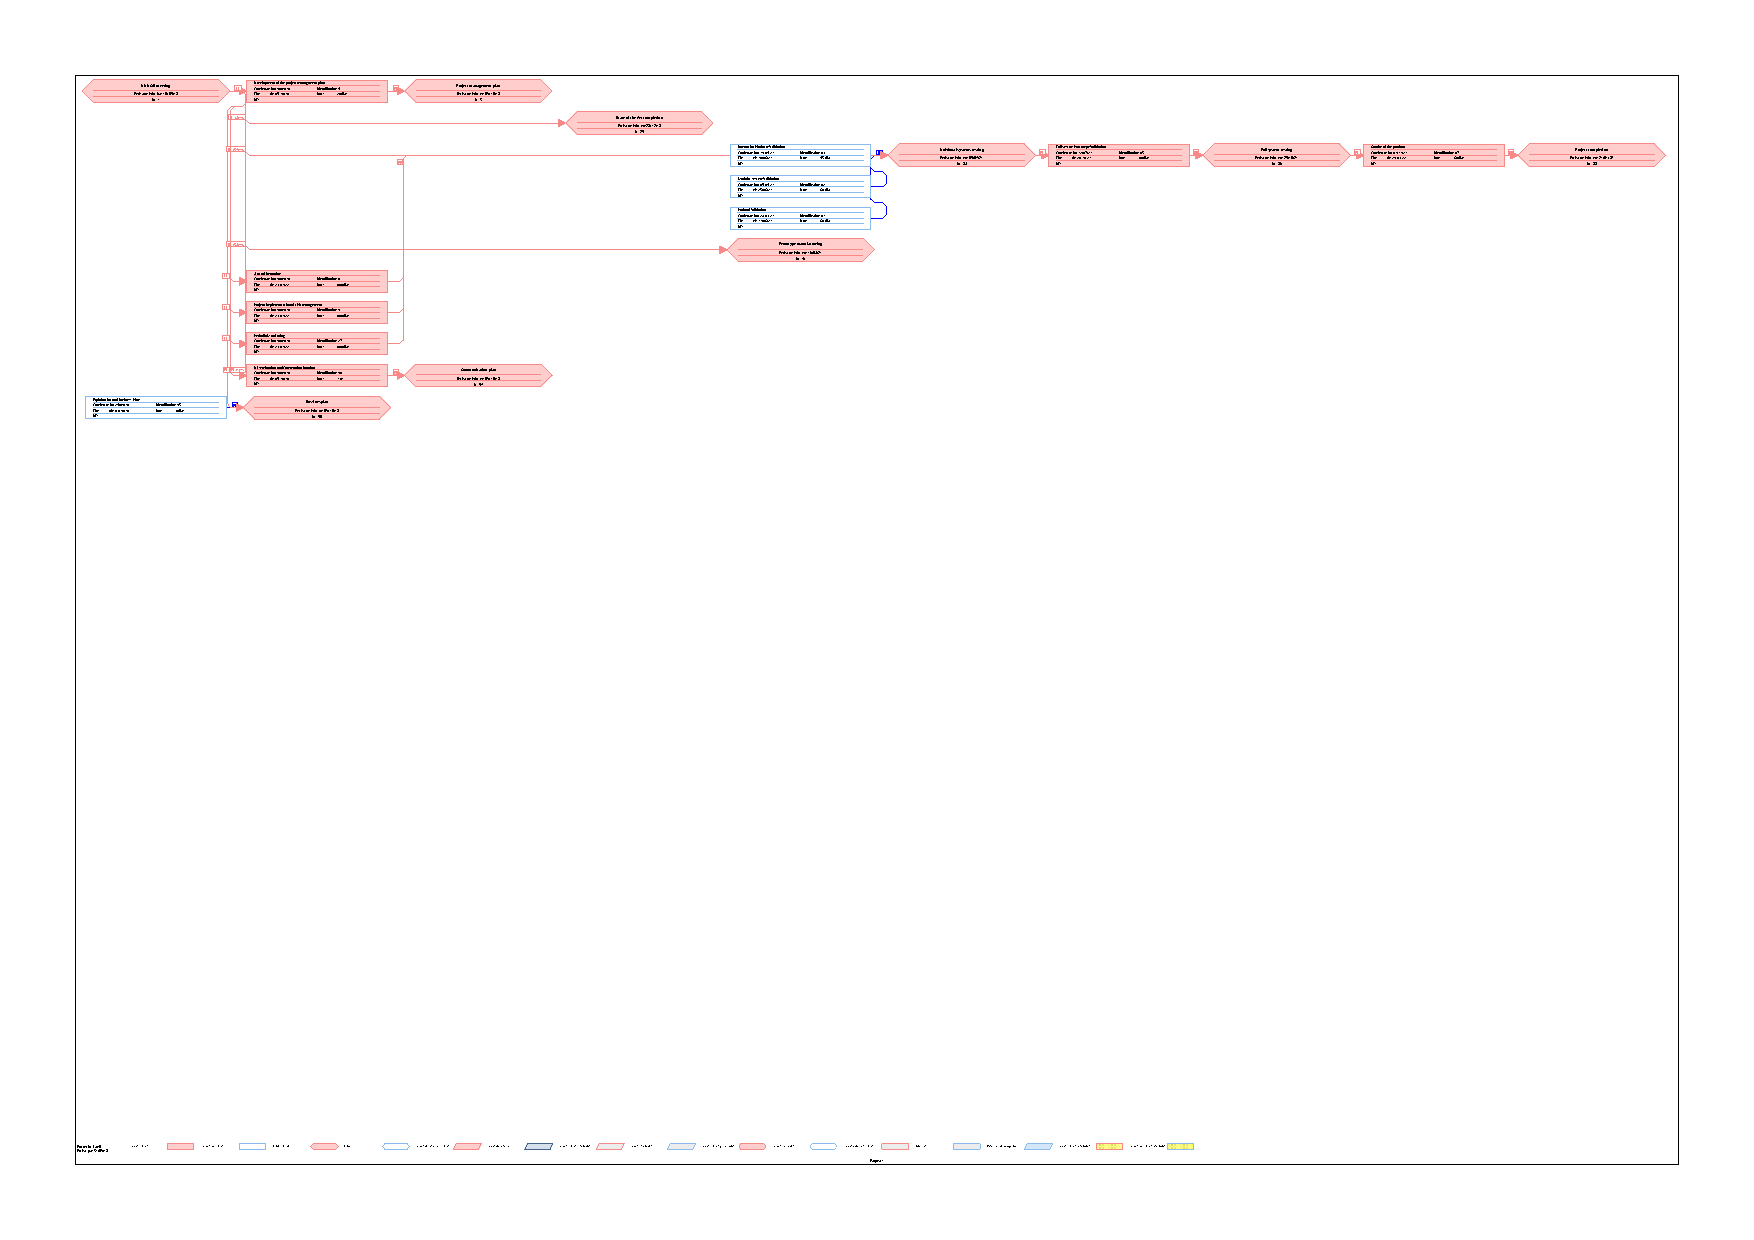
\includegraphics[page=1,width=1.2\textwidth]{./pdf/network.pdf}
	\end{tabular}
	\caption{Network diagram}
	\label{Gantt}
	\end{figure}
\end{landscape}